\documentclass{standalone}
\usepackage{tikz}
\usetikzlibrary{patterns, positioning}


\begin{document}
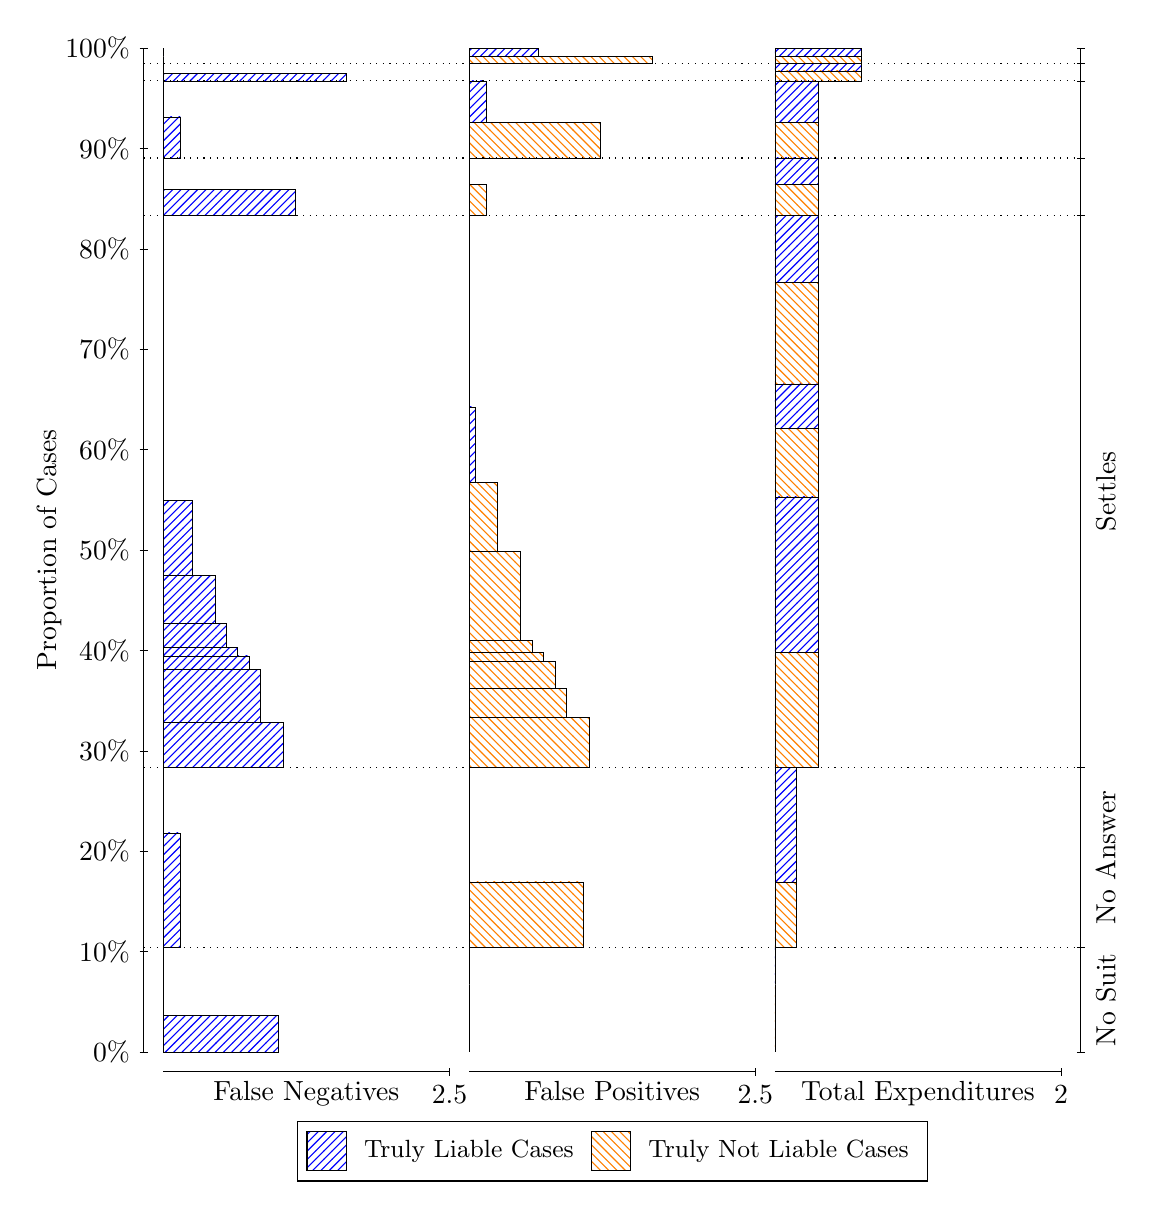
\begin{tikzpicture}
\draw[black, very thin] (1.5,1.75) -- (1.5,14.5);
\node[rotate=90, text=black, anchor=center] at (0.3, 8.125) {Proportion of Cases};
\draw[black, very thin] (1.45,1.75) -- (1.55,1.75);
\node[text=black, anchor=east] at (1.45, 1.75) {0\%};
\draw[black, very thin] (1.45,3.025) -- (1.55,3.025);
\node[text=black, anchor=east] at (1.45, 3.025) {10\%};
\draw[black, very thin] (1.45,4.3) -- (1.55,4.3);
\node[text=black, anchor=east] at (1.45, 4.3) {20\%};
\draw[black, very thin] (1.45,5.575) -- (1.55,5.575);
\node[text=black, anchor=east] at (1.45, 5.575) {30\%};
\draw[black, very thin] (1.45,6.85) -- (1.55,6.85);
\node[text=black, anchor=east] at (1.45, 6.85) {40\%};
\draw[black, very thin] (1.45,8.125) -- (1.55,8.125);
\node[text=black, anchor=east] at (1.45, 8.125) {50\%};
\draw[black, very thin] (1.45,9.4) -- (1.55,9.4);
\node[text=black, anchor=east] at (1.45, 9.4) {60\%};
\draw[black, very thin] (1.45,10.675) -- (1.55,10.675);
\node[text=black, anchor=east] at (1.45, 10.675) {70\%};
\draw[black, very thin] (1.45,11.95) -- (1.55,11.95);
\node[text=black, anchor=east] at (1.45, 11.95) {80\%};
\draw[black, very thin] (1.45,13.225) -- (1.55,13.225);
\node[text=black, anchor=east] at (1.45, 13.225) {90\%};
\draw[black, very thin] (1.45,14.5) -- (1.55,14.5);
\node[text=black, anchor=east] at (1.45, 14.5) {100\%};

\draw[black, very thin] (13.4,1.75) -- (13.4,14.5);
\draw[black, very thin] (13.35,1.75) -- (13.45,1.75);
\node[anchor=west] at (13.35, 1.75) {};
\draw[black, very thin] (13.35,3.0754) -- (13.45,3.0754);
\node[anchor=west] at (13.35, 3.0754) {};
\draw[black, very thin] (13.35,5.3667) -- (13.45,5.3667);
\node[anchor=west] at (13.35, 5.3667) {};
\draw[black, very thin] (13.35,12.374) -- (13.45,12.374);
\node[anchor=west] at (13.35, 12.374) {};
\draw[black, very thin] (13.35,13.104) -- (13.45,13.104);
\node[anchor=west] at (13.35, 13.104) {};
\draw[black, very thin] (13.35,14.082) -- (13.45,14.082);
\node[anchor=west] at (13.35, 14.082) {};
\draw[black, very thin] (13.35,14.308) -- (13.45,14.308);
\node[anchor=west] at (13.35, 14.308) {};
\draw[black, very thin] (13.35,14.5) -- (13.45,14.5);
\node[anchor=west] at (13.35, 14.5) {};

\draw[black, very thin, pattern color=blue, pattern=north east lines] (1.75,1.75) rectangle (3.2033,2.2171);
\draw[black, very thin, pattern color=orange, pattern=north west lines] (1.75,2.2171) rectangle (1.75,3.0754);
\draw[black, very thin, pattern color=blue, pattern=north east lines] (1.75,3.0754) rectangle (1.968,4.533);
\draw[black, very thin, pattern color=orange, pattern=north west lines] (1.75,4.533) rectangle (1.75,5.3667);
\draw[black, very thin, pattern color=blue, pattern=north east lines] (1.75,5.3667) rectangle (3.276,5.9309);
\draw[black, very thin, pattern color=blue, pattern=north east lines] (1.75,5.9309) rectangle (2.9853,6.6106);
\draw[black, very thin, pattern color=blue, pattern=north east lines] (1.75,6.6106) rectangle (2.84,6.781);
\draw[black, very thin, pattern color=blue, pattern=north east lines] (1.75,6.781) rectangle (2.6947,6.8908);
\draw[black, very thin, pattern color=blue, pattern=north east lines] (1.75,6.8908) rectangle (2.5493,7.195);
\draw[black, very thin, pattern color=blue, pattern=north east lines] (1.75,7.195) rectangle (2.404,7.7995);
\draw[black, very thin, pattern color=blue, pattern=north east lines] (1.75,7.7995) rectangle (2.1133,8.7587);
\draw[black, very thin, pattern color=orange, pattern=north west lines] (1.75,8.7587) rectangle (1.75,12.374);
\draw[black, very thin, pattern color=blue, pattern=north east lines] (1.75,12.374) rectangle (3.4213,12.707);
\draw[black, very thin, pattern color=orange, pattern=north west lines] (1.75,12.707) rectangle (1.75,13.104);
\draw[black, very thin, pattern color=blue, pattern=north east lines] (1.75,13.104) rectangle (1.968,13.626);
\draw[black, very thin, pattern color=orange, pattern=north west lines] (1.75,13.626) rectangle (1.75,14.082);
\draw[black, very thin, pattern color=blue, pattern=north east lines] (1.75,14.082) rectangle (4.0753,14.179);
\draw[black, very thin, pattern color=orange, pattern=north west lines] (1.75,14.179) rectangle (1.75,14.308);
\draw[black, very thin, pattern color=orange, pattern=north west lines] (1.75,14.308) rectangle (1.75,14.394);
\draw[black, very thin, pattern color=blue, pattern=north east lines] (1.75,14.394) rectangle (1.75,14.5);
\draw[black, very thin, pattern color=orange, pattern=north west lines] (5.6333,1.75) rectangle (5.6333,2.6083);
\draw[black, very thin, pattern color=blue, pattern=north east lines] (5.6333,2.6083) rectangle (5.6333,3.0754);
\draw[black, very thin, pattern color=orange, pattern=north west lines] (5.6333,3.0754) rectangle (7.0867,3.909);
\draw[black, very thin, pattern color=blue, pattern=north east lines] (5.6333,3.909) rectangle (5.6333,5.3667);
\draw[black, very thin, pattern color=orange, pattern=north west lines] (5.6333,5.3667) rectangle (7.1593,6.0018);
\draw[black, very thin, pattern color=orange, pattern=north west lines] (5.6333,6.0018) rectangle (6.8687,6.3703);
\draw[black, very thin, pattern color=orange, pattern=north west lines] (5.6333,6.3703) rectangle (6.7233,6.711);
\draw[black, very thin, pattern color=orange, pattern=north west lines] (5.6333,6.711) rectangle (6.578,6.8209);
\draw[black, very thin, pattern color=orange, pattern=north west lines] (5.6333,6.8209) rectangle (6.4327,6.973);
\draw[black, very thin, pattern color=orange, pattern=north west lines] (5.6333,6.973) rectangle (6.2873,8.1097);
\draw[black, very thin, pattern color=orange, pattern=north west lines] (5.6333,8.1097) rectangle (5.9967,8.9821);
\draw[black, very thin, pattern color=blue, pattern=north east lines] (5.6333,8.9821) rectangle (5.706,9.9412);
\draw[black, very thin, pattern color=blue, pattern=north east lines] (5.6333,9.9412) rectangle (5.6333,12.374);
\draw[black, very thin, pattern color=orange, pattern=north west lines] (5.6333,12.374) rectangle (5.8513,12.771);
\draw[black, very thin, pattern color=blue, pattern=north east lines] (5.6333,12.771) rectangle (5.6333,13.104);
\draw[black, very thin, pattern color=orange, pattern=north west lines] (5.6333,13.104) rectangle (7.3047,13.56);
\draw[black, very thin, pattern color=blue, pattern=north east lines] (5.6333,13.56) rectangle (5.8513,14.082);
\draw[black, very thin, pattern color=orange, pattern=north west lines] (5.6333,14.082) rectangle (5.6333,14.211);
\draw[black, very thin, pattern color=blue, pattern=north east lines] (5.6333,14.211) rectangle (5.6333,14.308);
\draw[black, very thin, pattern color=orange, pattern=north west lines] (5.6333,14.308) rectangle (7.9587,14.394);
\draw[black, very thin, pattern color=blue, pattern=north east lines] (5.6333,14.394) rectangle (6.5053,14.5);
\draw[black, very thin, pattern color=orange, pattern=north west lines] (9.5167,1.75) rectangle (9.5167,2.6083);
\draw[black, very thin, pattern color=blue, pattern=north east lines] (9.5167,2.6083) rectangle (9.5167,3.0754);
\draw[black, very thin, pattern color=orange, pattern=north west lines] (9.5167,3.0754) rectangle (9.7892,3.909);
\draw[black, very thin, pattern color=blue, pattern=north east lines] (9.5167,3.909) rectangle (9.7892,5.3667);
\draw[black, very thin, pattern color=orange, pattern=north west lines] (9.5167,5.3667) rectangle (10.062,6.8209);
\draw[black, very thin, pattern color=blue, pattern=north east lines] (9.5167,6.8209) rectangle (10.062,8.7986);
\draw[black, very thin, pattern color=orange, pattern=north west lines] (9.5167,8.7986) rectangle (10.062,9.671);
\draw[black, very thin, pattern color=blue, pattern=north east lines] (9.5167,9.671) rectangle (10.062,10.235);
\draw[black, very thin, pattern color=orange, pattern=north west lines] (9.5167,10.235) rectangle (10.062,11.524);
\draw[black, very thin, pattern color=blue, pattern=north east lines] (9.5167,11.524) rectangle (10.062,12.374);
\draw[black, very thin, pattern color=orange, pattern=north west lines] (9.5167,12.374) rectangle (10.062,12.771);
\draw[black, very thin, pattern color=blue, pattern=north east lines] (9.5167,12.771) rectangle (10.062,13.104);
\draw[black, very thin, pattern color=orange, pattern=north west lines] (9.5167,13.104) rectangle (10.062,13.56);
\draw[black, very thin, pattern color=blue, pattern=north east lines] (9.5167,13.56) rectangle (10.062,14.082);
\draw[black, very thin, pattern color=orange, pattern=north west lines] (9.5167,14.082) rectangle (10.607,14.211);
\draw[black, very thin, pattern color=blue, pattern=north east lines] (9.5167,14.211) rectangle (10.607,14.308);
\draw[black, very thin, pattern color=orange, pattern=north west lines] (9.5167,14.308) rectangle (10.607,14.394);
\draw[black, very thin, pattern color=blue, pattern=north east lines] (9.5167,14.394) rectangle (10.607,14.5);
\draw[black, dotted] (1.5,3.0754) -- (13.4,3.0754);
\draw[black, dotted] (1.5,5.3667) -- (13.4,5.3667);
\draw[black, dotted] (1.5,12.374) -- (13.4,12.374);
\draw[black, dotted] (1.5,13.104) -- (13.4,13.104);
\draw[black, dotted] (1.5,14.082) -- (13.4,14.082);
\draw[black, dotted] (1.5,14.308) -- (13.4,14.308);
\draw[black, very thin] (1.75,1.5) -- (5.3833,1.5);
\node[text=black, anchor=north] at (3.5667, 1.5) {False Negatives};
\draw[black, very thin] (5.3833,1.45) -- (5.3833,1.55);
\node[text=black, anchor=north] at (5.3833, 1.45) {2.5};

\draw[black, very thin] (5.6333,1.5) -- (9.2667,1.5);
\node[text=black, anchor=north] at (7.45, 1.5) {False Positives};
\draw[black, very thin] (9.2667,1.45) -- (9.2667,1.55);
\node[text=black, anchor=north] at (9.2667, 1.45) {2.5};

\draw[black, very thin] (9.5167,1.5) -- (13.15,1.5);
\node[text=black, anchor=north] at (11.333, 1.5) {Total Expenditures};
\draw[black, very thin] (13.15,1.45) -- (13.15,1.55);
\node[text=black, anchor=north] at (13.15, 1.45) {2};

\node[text=black, centered, rotate=90] at (13.72, 2.4127) {No Suit};
\node[text=black, centered, rotate=90] at (13.72, 4.221) {No Answer};
\node[text=black, centered, rotate=90] at (13.72, 8.8704) {Settles};





\draw (7.449999999999999,1.5) node[draw=none] (baseCoordinate) {};
\begin{scope}[align=center]
        \matrix[scale=0.5, draw=black, below=0.5cm of baseCoordinate, nodes={draw}, column sep=0.1cm]{
            \node[rectangle, draw, minimum width=0.5cm, minimum height=0.5cm, pattern color=blue, pattern=north east lines] {}; &
            \node[draw=none, font=\small, text=black] (B) {Truly Liable Cases}; &
            \node[rectangle, draw, minimum width=0.5cm, minimum height=0.5cm, pattern color=orange, pattern=north west lines] {}; &
            \node[draw=none, font=\small, text=black] (B) {Truly Not Liable Cases}; \\
            };
\end{scope}

\end{tikzpicture}
\end{document}